\chapter{O Método dos Elementos Finitos}

\begin{quote}
    "As far as the laws of mathematics refer to reality, they are not certain; and as far as they are certain, they do not refer to reality." (Albert Einstein)
\end{quote}


O Método dos Elementos Finitos (MEF), \emph{Finite Element Method} (FEM), é um método numérico, e tem como finalidade aproximar a solução de funções de campo numericamente, o domínios que são difíceis de se obter repostas diretas algebricamente. Para tanto, esse domínio é discretizado em vários elementos, ou sub-domínios, de tamanho finito, cujos comportamentos já são conhecidos da aplicação de leis físicas. A função de campo desconhecida é aproximada em cada elemento por meio de funções interpoladoras, calculadas sobre o valor de campo em cada nó, que são os pontos do domínio sobre os quais os elementos são construídos (o campo, portanto, passa a ser definido não mais pelo conjunto de valores do contínuo, mais sim por essas variáveis desconhecidas discretizadas). Para cada elemento, são definidas equações, por meio das quais eles se relacionam entre si e com o campo. Isso leva à formação de um grande sistema linear, que pode ser resolvido facilmente, e obter-se, dessa forma, a aproximação da função de campo. \cite{Onate}

\begin{figure}
	\centering
    \caption{Domínio discretizado em elementos triangulares.}
    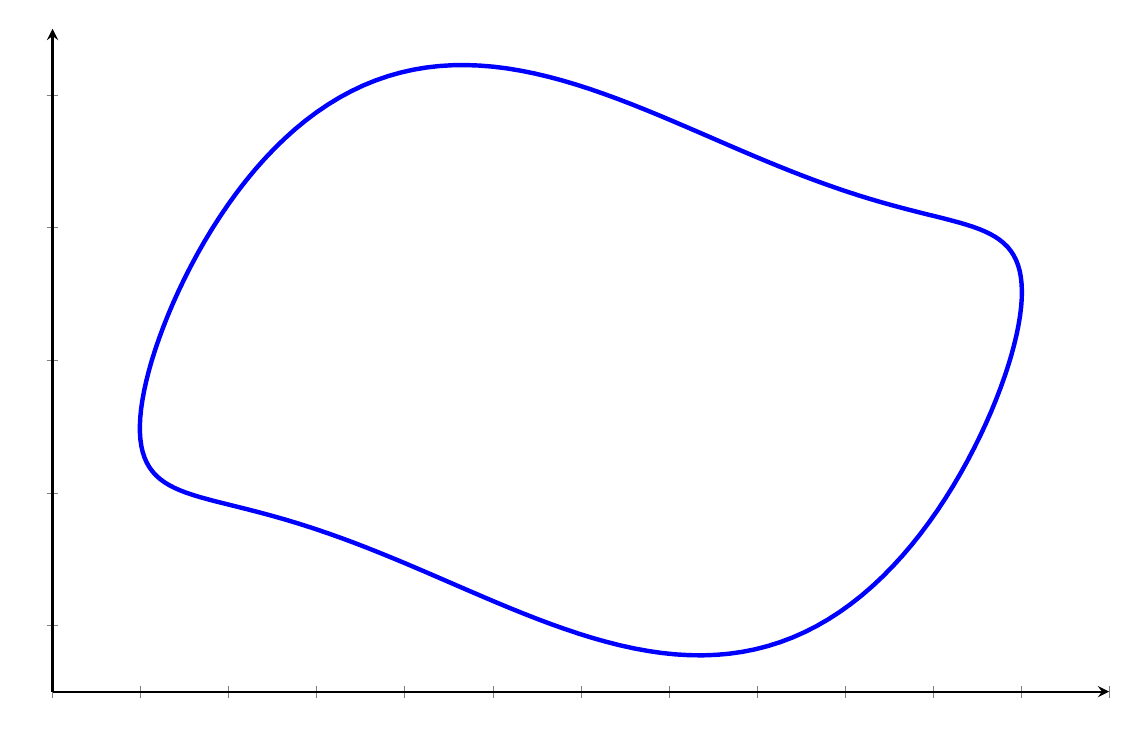
\begin{tikzpicture}
        \begin{axis}[
                xmin = -6, xmax = 6,
                ymin = -2.5, ymax = 2.5,
                height = 10 cm, width = 15 cm,
                axis lines = left,
                xticklabels = {,,},
                yticklabels = {,,},
                axis line style = thick
            ]
            \addplot[domain=0:360,samples=200, blue, ultra thick]({5 * cos(x) + 0.3 * sin(x)},{2 * sin(x) + 0.4 * cos(3 *x)});
        \end{axis}
    \end{tikzpicture}
	\fonte{\me{2022}}
\end{figure}